% ------------------------------------------------------------------------------
% TYPO3 CMS 8.5 - What's New - Chapter "In-Depth Changes" (English Version)
%
% @author	Michael Schams <schams.net>
% @license	Creative Commons BY-NC-SA 3.0
% @link		http://typo3.org/download/release-notes/whats-new/
% @language	English
% ------------------------------------------------------------------------------
% LTXE-CHAPTER-UID:		5ebcecbe-66abfa57-cf38bc00-aa637965
% LTXE-CHAPTER-NAME:	In-Depth Changes
% ------------------------------------------------------------------------------

\section{In-Depth Changes}
\begin{frame}[fragile]
	\frametitle{In-Depth Changes}

	\begin{center}\huge{Chapter 3:}\end{center}
	\begin{center}\huge{\color{typo3darkgrey}\textbf{In-Depth Changes}}\end{center}

\end{frame}

% ------------------------------------------------------------------------------
% LTXE-SLIDE-START
% LTXE-SLIDE-UID:		bde270e6-ffef8544-ea472ed5-89ba8c3d
% LTXE-SLIDE-TITLE:		#78581: FormEngine Data Providers
% ------------------------------------------------------------------------------

\begin{frame}[fragile]
	\frametitle{In-Depth Changes}
	\framesubtitle{FormEngine Data Providers}

	\begin{itemize}
		\item FormEngine data provider \texttt{TcaFlexFetch} has been merged into \texttt{TcaFlexPrepare}
		\item This only affects instances in the unlikely case that a custom data provider declared a
			dependency to \texttt{TcaFlexFetch}
	\end{itemize}

\end{frame}

% ------------------------------------------------------------------------------
% LTXE-SLIDE-START
% LTXE-SLIDE-UID:		f0fb603c-54e9f255-03140395-b6b18103
% LTXE-SLIDE-TITLE:		#78384: Frontend ignores TCA in ext_tables.php
% ------------------------------------------------------------------------------
\begin{frame}[fragile]
	\frametitle{In-Depth Changes}
	\framesubtitle{TCA in \texttt{ext\_tables.php}}

	\begin{itemize}
		\item Frontend requests no longer load \texttt{ext\_tables.php} in requests
		\item This change impacts extensions which configure the TCA in \texttt{ext\_tables.php}\newline
			\small(which is not allowed anyway)\normalsize
		\item Install Tool provides a test "TCA ext\_tables check" to identify such extensions
	\end{itemize}

	\begin{figure}
		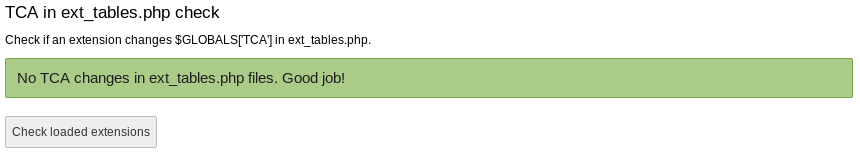
\includegraphics[width=0.95\linewidth]{InDepthChanges/78384-install-tool-tca-in-exttables-check.png}
	\end{figure}

\end{frame}
% ------------------------------------------------------------------------------
% LTXE-SLIDE-START
% LTXE-SLIDE-UID:		bdcd2449-b679717b-9f23eb32-018953b4
% LTXE-SLIDE-TITLE:		#78191: Remove support for transForeignTable/transOrigPointerTable in TCA
% ------------------------------------------------------------------------------
\begin{frame}[fragile]
	\frametitle{In-Depth Changes}
	\framesubtitle{TCA in \texttt{ext\_tables.php}}

	\begin{itemize}
		\item Database tables which hold localized and translated records were configurable in the TCA

			\begin{itemize}
				\item \texttt{\$TCA[<table\_name>]['ctrl']['transForeignTable']}\newline
					(usually pointed to table: \texttt{pages\_language\_overlay})
				\item \texttt{\$TCA[<table\_name>]['ctrl']['transOrigPointerTable']}\newline
					(usually pointed to table: \texttt{pages})
			\end{itemize}

		\item This configuration has been replaced with hard-coded table names in order to prevent
			special handling and prepare for a combination of both tables in the future

	\end{itemize}

\end{frame}

% ------------------------------------------------------------------------------
% LTXE-SLIDE-START
% LTXE-SLIDE-UID:		ede02440-cafd3417-eb416f09-8e024ef2
% LTXE-SLIDE-TITLE:		#78383: Tables removed from defaultCategorizedTables
% ------------------------------------------------------------------------------
\begin{frame}[fragile]
	\frametitle{In-Depth Changes}
	\framesubtitle{Tables removed from \texttt{defaultCategorizedTables}}

	\begin{itemize}
		\item The following tables have been removed from \texttt{defaultCategorizedTables}:

			\begin{itemize}
				\item \texttt{pages}
				\item \texttt{tt\_content}
				\item \texttt{sys\_file\_metadata}
			\end{itemize}

		\item For these tables the core API\newline
			\texttt{ExtensionManagementUtility::makeCategorizable()}\newline
			is executed to define a common position of the categories field

	\end{itemize}

\end{frame}


% ------------------------------------------------------------------------------
% LTXE-SLIDE-START
% LTXE-SLIDE-UID:		dd31e5d5-ca09ae5e-eb87d926-0ffe8f0a
% LTXE-SLIDE-TITLE:		Low-level parameters changes (1)
% ------------------------------------------------------------------------------
\begin{frame}[fragile]
	\frametitle{In-Depth Changes}
	\framesubtitle{Low-level Parameter Changes (1)}

	% changes: #78417, #78439, #78520, #78552, #78577, #78623, #78627 and #78895

	\begin{itemize}
		\item Low-level commands listed below use the Symfony Console now
		\item New commands behave like the old ones, but allow using certain parameters

			\begin{itemize}
				\item \texttt{DeletedRecordsCommand}
				\item \texttt{CleanFlexFormsRecordsCommand}
				\item \texttt{OrphanRecordsCommand}
				\item \texttt{LostFilesCommand}
				\item \texttt{MissingFilesCommand}
				\item \texttt{MissingRelationsCommand}
				\item \texttt{DoubleFilesCommand}
				\item \texttt{RteImagesCommand}
			\end{itemize}

	\end{itemize}

\end{frame}



% ------------------------------------------------------------------------------
% LTXE-SLIDE-START
% LTXE-SLIDE-UID:		3a9d25bb-d948368d-e2a92666-6170eaad
% LTXE-SLIDE-TITLE:		Low-level parameters changes (2)
% ------------------------------------------------------------------------------
\begin{frame}[fragile]
	\frametitle{In-Depth Changes}
	\framesubtitle{Low-level Parameter Changes (2)}

	% changes: #78417, #78439, #78520, #78552, #78577, #78623, #78627 and #78895

	\begin{itemize}
		\item Related PHP classes have been removed\newline
			\smaller(e.g. \texttt{TYPO3\textbackslash
				CMS\textbackslash
				Lowlevel\textbackslash
				DeletedRecordsCommand})
			\normalsize

		\item Executing the command via \texttt{cli\_dispatch} does not work anymore\newline
			\smaller(e.g. \texttt{typo3/cli\_dispatch lowlevel cleaner deleted})\normalsize
		\item Calling the PHP class results in a fatal PHP error now

		\item Commands can now be executed via CLI as follows:\newline
			\smaller\texttt{/typo3/sysext/core/bin/typo3 cleanup:<command>}\normalsize\newline
			for example:\newline
			\smaller\texttt{/typo3/sysext/core/bin/typo3 cleanup:deletedrecords}\normalsize

	\end{itemize}

\end{frame}




% ------------------------------------------------------------------------------
% LTXE-SLIDE-START
% LTXE-SLIDE-UID:		ec6817fd-c3364ffb-c74e9523-a18a3095
% LTXE-SLIDE-TITLE:		Re-factor FlexForm Data Structure Handling
% ------------------------------------------------------------------------------
\begin{frame}[fragile]
	\frametitle{In-Depth Changes}
	\framesubtitle{Re-factor FlexForm Data Structure Handling}

	% https://forge.typo3.org/issues/78581
	% https://forge.typo3.org/issues/78616
	% https://forge.typo3.org/issues/78852
	% https://forge.typo3.org/issues/69715

	\begin{itemize}
		\item With the deprecation of \texttt{BackendUtility::getFlexFormDS()} the hook
			\texttt{getFlexFormDSClass} is no longer called

	\end{itemize}

\end{frame}





% ------------------------------------------------------------------------------
% LTXE-SLIDE-START
% LTXE-SLIDE-UID:		b400c3b8-3e402480-cd7d6ff3-96cd93aa
% LTXE-SLIDE-TITLE:		#76085: Add fluid debug information to admin panel
% ------------------------------------------------------------------------------
\begin{frame}[fragile]
	\frametitle{In-Depth Changes}
	\framesubtitle{Admin Panel}

	\begin{itemize}
		\item Admin Panel features a new setting to debug Fluid output:\newline
			\textbf{Preview -> Show fluid debug output}
		\item If enabled, the following details are shown in the frontend:

			\begin{itemize}
				\item path to the template file of a partial
				\item name of a section
			\end{itemize}

		\item This feature enables integrators to easily locate the correct template and section

	\end{itemize}

\end{frame}






% ------------------------------------------------------------------------------
% LTXE-SLIDE-START
% LTXE-SLIDE-UID:		60a2d39f-f04b8bf1-dc758912-607ed07e
% LTXE-SLIDE-TITLE:		#52286: System Status Updates Report via email
% ------------------------------------------------------------------------------
\begin{frame}[fragile]
	\frametitle{In-Depth Changes}
	\framesubtitle{System Status Updates (Reports)}

	\begin{itemize}
		\item Results of test in the "System Status Updates (reports)" can be sent via email
		\item A checkbox has been added to the job configuration to:

			\begin{itemize}
				\item send an email if the system has warnings or errors
				\item always generate an email
			\end{itemize}

		\item The default is to include warnings and errors only

	\end{itemize}

\end{frame}







% ------------------------------------------------------------------------------
% LTXE-SLIDE-START
% LTXE-SLIDE-UID:		e4e2ead3-c07beb21-e8100580-d0e7c756
% LTXE-SLIDE-TITLE:		#58637: Purge language packs in language module
% ------------------------------------------------------------------------------
\begin{frame}[fragile]
	\frametitle{In-Depth Changes}
	\framesubtitle{Language Packs}

	\begin{itemize}
		\item Deactivating languages in the module "Languages" left language data remaining
			in directory \texttt{typo3conf/l10n/<locale>/}
		\item A "remove"-button has been added, which disables the language and purges the
			data in the directory
	\end{itemize}

\end{frame}








% ------------------------------------------------------------------------------
% LTXE-SLIDE-START
% LTXE-SLIDE-UID:		08961fb3-00cbc9f4-964f8d01-6e59e782
% LTXE-SLIDE-TITLE:		#67909: Hook added to localize() function
% ------------------------------------------------------------------------------
\begin{frame}[fragile]
	\frametitle{In-Depth Changes}
	\framesubtitle{Hook in DataHandler \texttt{localize()}}

	% decrease font size for code listing
	\lstset{basicstyle=\tiny\ttfamily}

	\begin{itemize}
		\item A new hook has been added to the \texttt{localize()} function
		\item This allows for example to use external translation services or custom transliteration
			functions that handle various content transformations
	\end{itemize}

	\begin{itemize}
		\item Hook:\newline
			\smaller
				\texttt{\$GLOBALS['TYPO3\_CONF\_VARS']['SC\_OPTIONS']\newline
				\tabto{0.4cm}['t3lib/class.t3lib\_tcemain.php']['processTranslateToClass']}
			\normalsize

		\item Example usage:

			\begin{lstlisting}
				class YourHookClass
				{
				  public function processTranslateTo_copyAction(&$content, $lang, $dataHandler)
				  {
				    // Do something with content (translate, transliterate etc.)
				  }
				}
			\end{lstlisting}
	\end{itemize}

\end{frame}









% ------------------------------------------------------------------------------
% LTXE-SLIDE-START
% LTXE-SLIDE-UID:		8b1a9661-d6fab90f-9c856224-ee663aa2
% LTXE-SLIDE-TITLE:		#77757: Re-check if an UpdateWizard should run
% ------------------------------------------------------------------------------
\begin{frame}[fragile]
	\frametitle{In-Depth Changes}
	\framesubtitle{Update Wizard}

	\begin{columns}[T]
		\begin{column}{.5\textwidth}
			The Update Wizard in the Install Tool lists all tasks marked as \textit{completed}.
			\newline\newline
			Checkboxes and a button "Recheck chosen wizards" allow to re-initiate the updates.
			The wizard will test if the task needs to be executed again.
		\end{column}
		\begin{column}{.5\textwidth}
			\begin{figure}\vspace*{-0.5cm}
				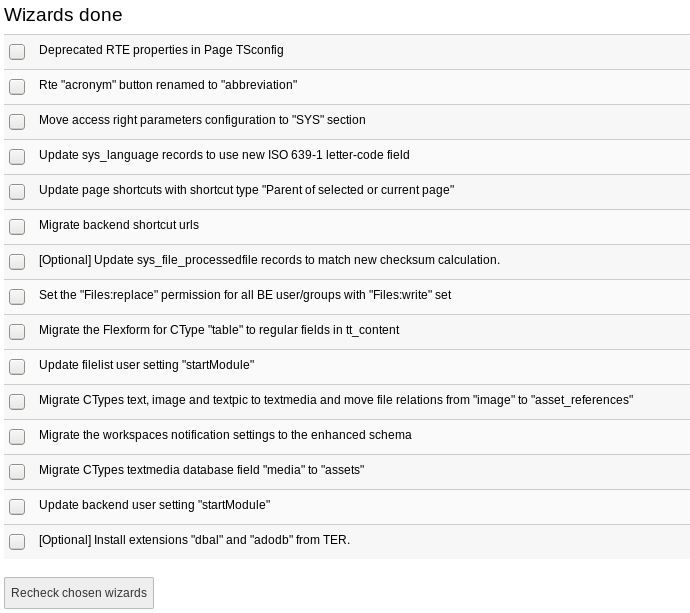
\includegraphics[width=0.8\linewidth]{InDepthChanges/77757-upgrade-wizard.png}
			\end{figure}
		\end{column}
	\end{columns}

\end{frame}









% ------------------------------------------------------------------------------
% LTXE-SLIDE-START
% LTXE-SLIDE-UID:		94640f3d-0f632507-a2166719-5adc755e
% LTXE-SLIDE-TITLE:		#78523: Suggest wizard provides option to define ordering of results
% ------------------------------------------------------------------------------
\begin{frame}[fragile]
	\frametitle{In-Depth Changes}
	\framesubtitle{Suggest Wizard}

	% decrease font size for code listing
	\lstset{basicstyle=\tiny\ttfamily}

	\begin{itemize}
		\item The FormEngine ("TCEforms") allows to configure the order of results by the suggest wizard
		\item The new option is a standard SQL order-by definition:\newline
			\small\texttt{'orderBy' => 'field ASC/DESC'}\normalsize
		\item Example TCA configuration:

			\begin{lstlisting}
				'config' => [
				  ...
				  'wizards' => [
				    'suggest' => [
				      'type' => 'suggest',
				      'default' => [
				        'searchWholePhrase' => true,
				        'addWhere' => ' AND tx_news_domain_model_news.uid != ###THIS_UID###',
				        'orderBy => 'datetime DESC',
				      ]
				    ],
				  ],
				]
			\end{lstlisting}

	\end{itemize}

\end{frame}











% ------------------------------------------------------------------------------
% LTXE-SLIDE-START
% LTXE-SLIDE-UID:		0907e5d3-a12751cb-23f49488-7a05a208
% LTXE-SLIDE-TITLE:		Miscellaneous
% ------------------------------------------------------------------------------
\begin{frame}[fragile]
	\frametitle{In-Depth Changes}
	\framesubtitle{Miscellaneous}

	% #78103: Add missing information status for addSystemMessage
	% #78575: Get enumeration constants
	% #75232: Spread TypeConverter priorities

	\begin{itemize}
		\item All system information added by \texttt{addSystemInformation()} have
			\texttt{InformationStatus::STATUS\_NOTICE} as the default value now
		\item Enumeration constants can be retrieved easily now:

			\begin{itemize}
				\item \texttt{EnumerationClass::getName(\$value);}
				\item \texttt{EnumerationClass::getHumanReadableName(\$value);}
			\end{itemize}

		\item Priorities of core TypeConverters have changed from\newline
			\texttt{1}, \texttt{2}, \texttt{3},... to \texttt{10}, \texttt{20}, \texttt{30},...
			When registering custom TypeConverter(s), make sure they are using the correct priorities.

		\item \href{https://en.wikipedia.org/wiki/ISO_8601}{ISO-8601} is used to pass date and datetime
			values between server and client now. Check if your custom FormEngine render types need to
			be updated (\texttt{eval=date/datetime}).

	\end{itemize}

\end{frame}












% ------------------------------------------------------------------------------
